\begin{abstract}
Large language models (LLMs) have demonstrated impressive capabilities in a wide range of downstream natural language processing tasks. 
Nevertheless, their considerable sizes and memory demands hinder practical deployment, underscoring the importance of developing efficient compression strategies. 
Singular value decomposition (SVD) decomposes a matrix into orthogonal components, enabling efficient low-rank approximation. This is particularly suitable for LLM compression, where weight matrices often exhibit significant redundancy.
However, current SVD-based methods neglect the residual matrix from truncation, resulting in significant truncation loss. 
Additionally, compressing all layers of the model results in severe error propagation. 
To overcome these limitations, we propose \textbf{ERC-SVD}, a new post-training SVD-based LLM compression method from an error-controlled perspective. 
Specifically, we leverage the residual matrix generated during the truncation process to reduce truncation loss. 
Moreover, under a fixed overall compression ratio, we selectively compress the last few layers of the model, which mitigates error propagation and improves compressed model performance.
Comprehensive evaluations on diverse LLM families and multiple benchmark datasets indicate that ERC-SVD consistently achieves superior performance over existing counterpart methods, demonstrating its practical effectiveness.

{\renewcommand\twocolumn[1][]{#1}
\begin{center}
    \centering
    \renewcommand{\arraystretch}{0.05} %
    \vspace{-2mm}
    \begin{tabular}{c}
        \hspace{-1.6cm}
        % , height = 0.35\linewidth
        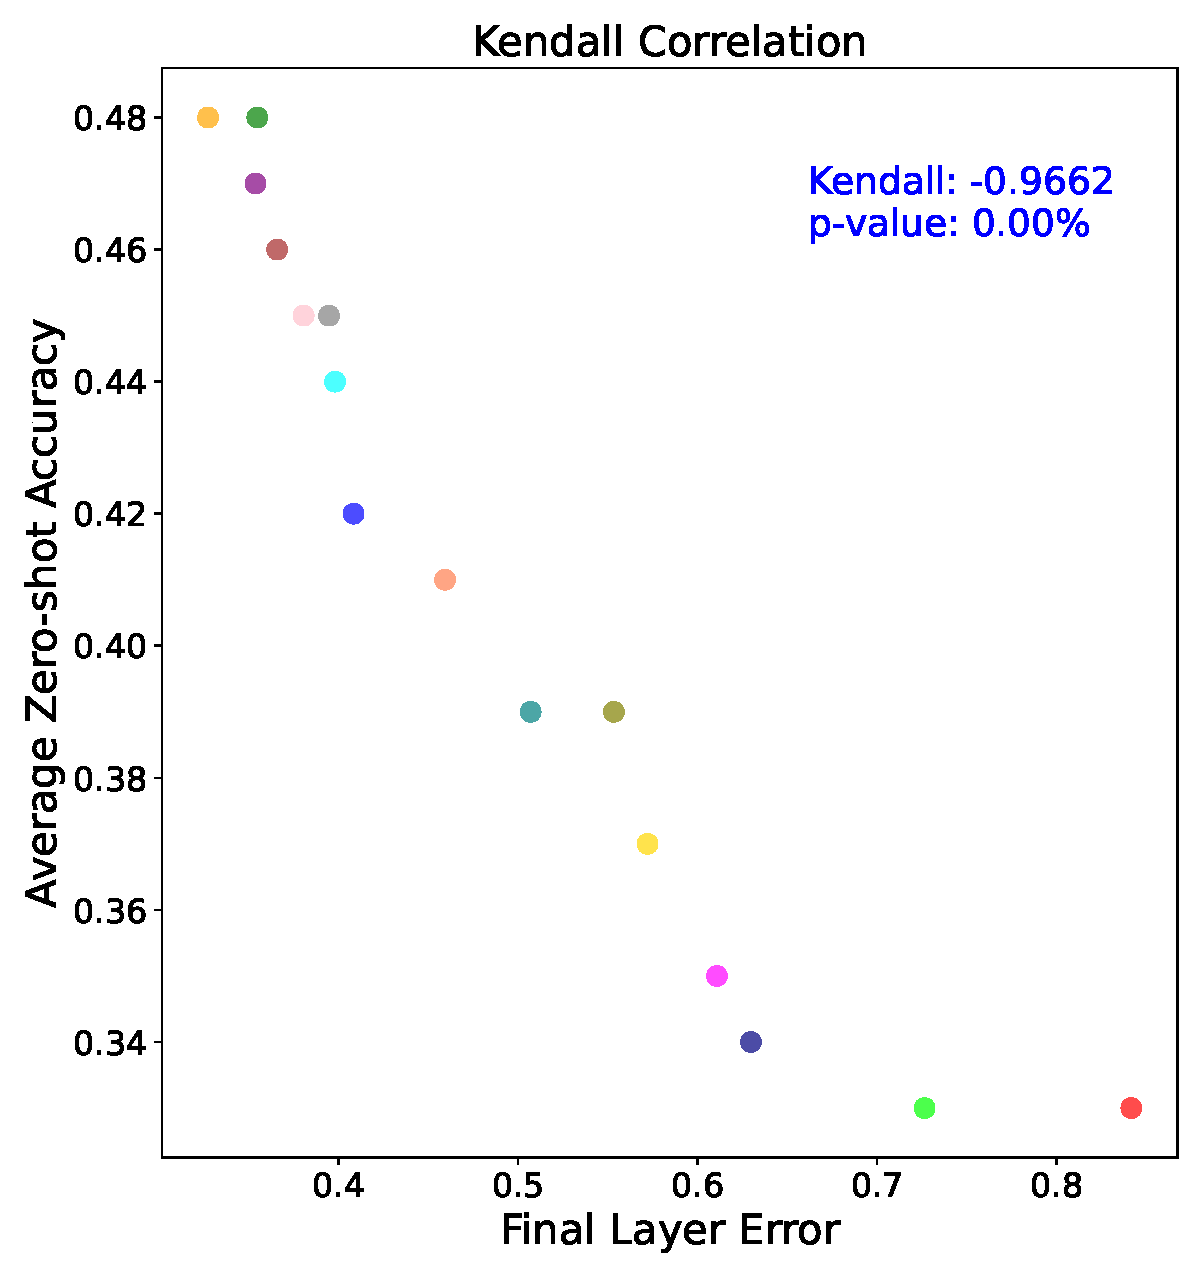
\includegraphics[width = 0.39\linewidth]{CPAL-2025-template/a_figures/kendall.pdf} 
        \hspace{0cm}
        % ,height = 0.3\linewidth
        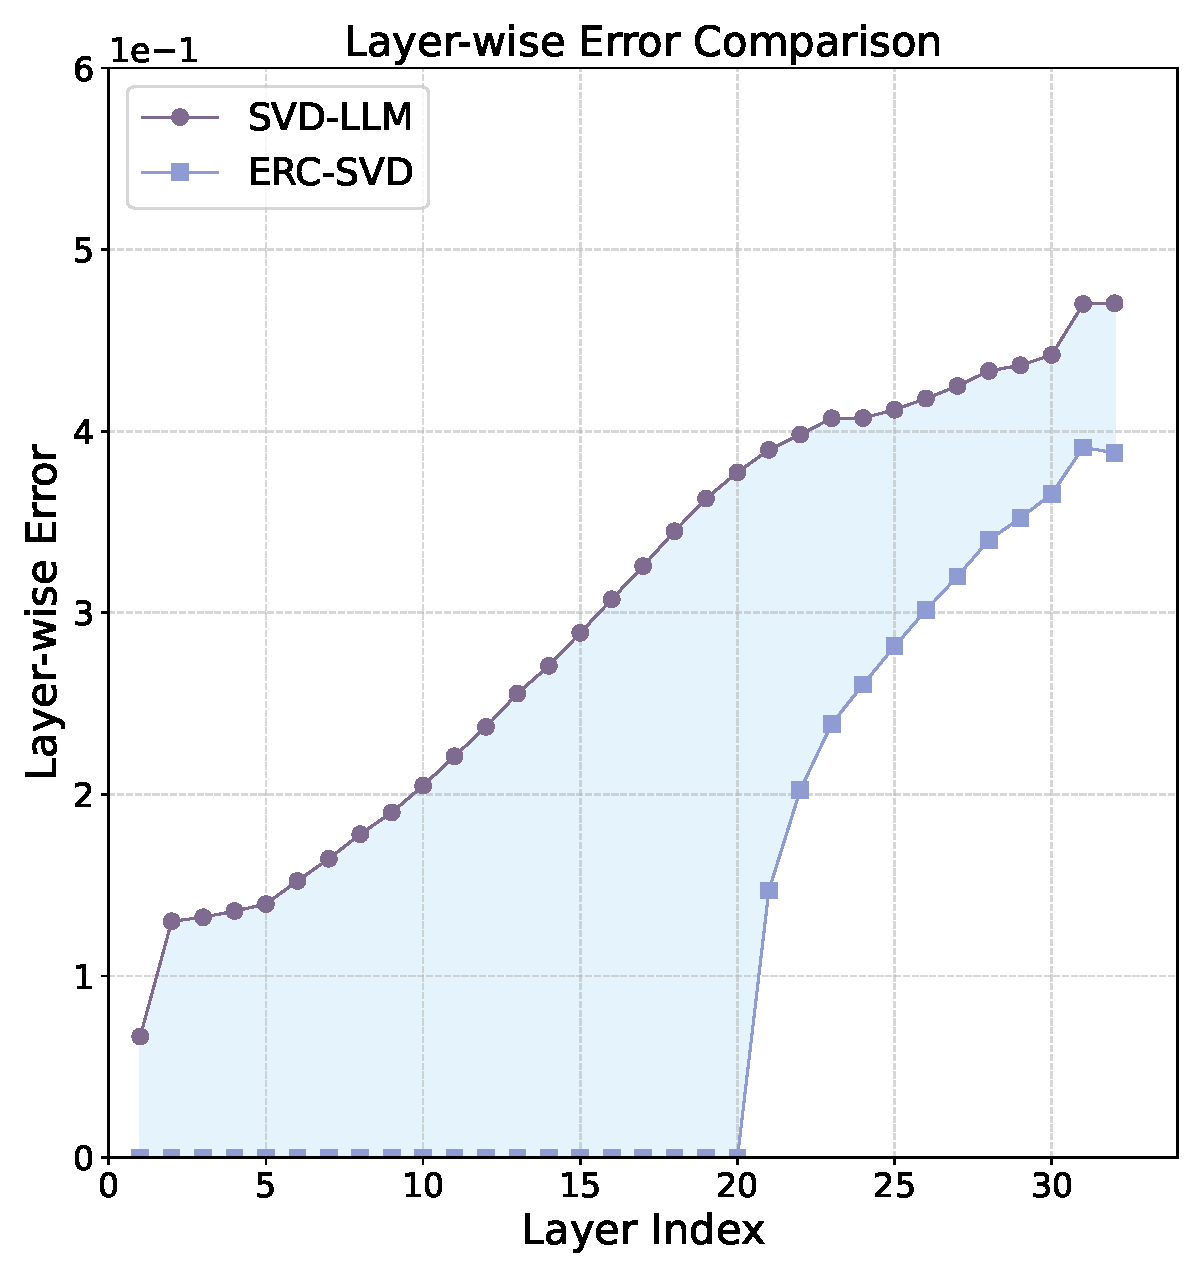
\includegraphics[width = 0.39\linewidth]{CPAL-2025-template/a_figures/layer_wise_loss_comparison.pdf}
        \hspace{0cm}
        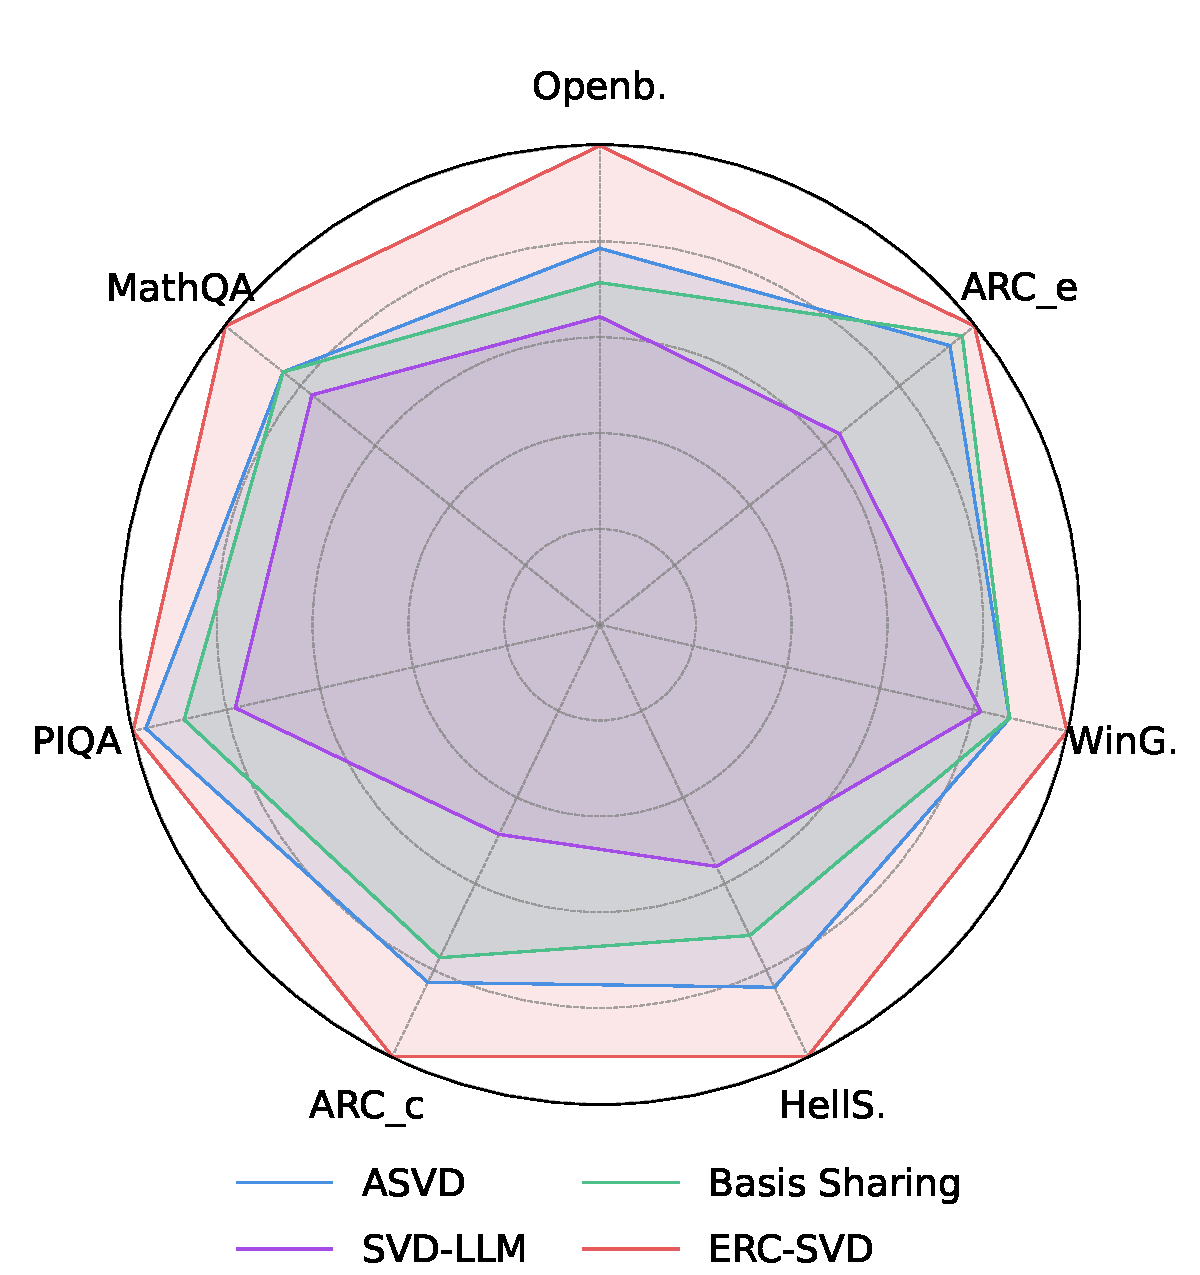
\includegraphics[width = 0.39\linewidth]{CPAL-2025-template/a_figures/rader.pdf}
        \end{tabular}
        \captionof{figure}{Left: The Kendall correlation between the final-layer error and the average zero-shot accuracy. Middle: Layer-wise error comparison between ERC-SVD and SVD-LLM of LLaMA-2-7B under 20\% compression ratio. Right: The accuracy comparison of LLaMA-2-7B compressed by different methods under 20\% compression ratio on seven reasoning and understanding tasks.}
    \label{fig:teaser}
\end{center}
}
\end{abstract}